\subsection{Quantitative data}

    %What the data said

    Two workshops were held, which together would inform future development of an application. These were the findings from those two workshops:

    \subsubsection{Customer Journey Map: "A day as a coach"}

    The first workshop had the tree interviewed coaches as participants. See figure \ref{fig:cjm}. A Customer Journey Map would be created, with the purpose to understand all activities involving “A day as a coach”. The structure of the timeline was: “Before”, “During”, and “After” a youth session. Too understand how these activities differentiated between different coaches, three Personas were co-created based on the previously dicovered types of coaches: "the ideal coach" (John), "the realistic coach" (Joan), and "the challenged coach" (Suzan).

    \begin{figure}[h]
        \centering
        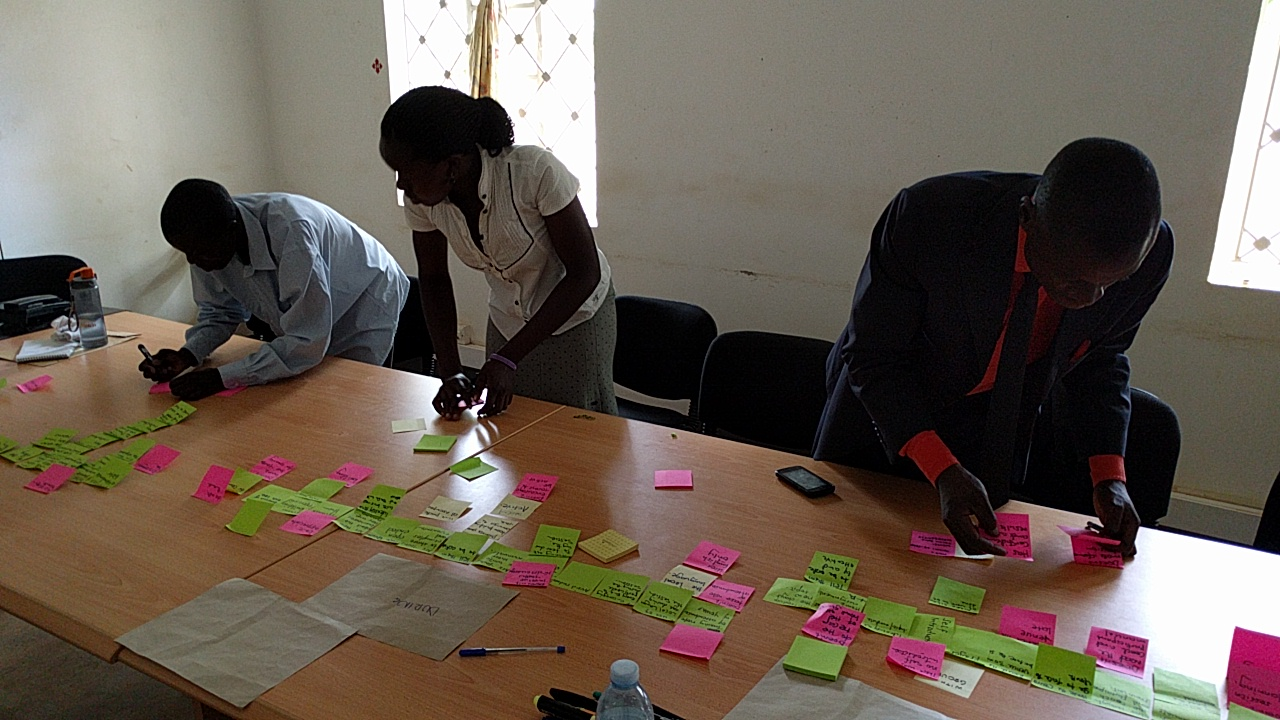
\includegraphics[width=0.7\textwidth]{cjmWorkshop.jpg}
        \caption{Two local project leaders and one coach mapping out the activities a coach does before, during and after hosting a youth session, in what is called a Customer Journey Map.}
        \label{fig:cjm}
    \end{figure}

    %After the 15 minute introduction, they started with 5 minutes + 10 minutes discussion mapping out Before, During, After for the ideal coach, John. Green postits were used.

    %Since it took too much time to do this for the other two personas, they were given 5 minutes to either use pink post-its for steps that a realistic coach would skip, and yellow notes that the coach would do differently. This worked well, and the results were discussed within the 5 minutes between the coaches, and explained during 5 minutes witth audio recording.

    %Since they were understandingly tired, they were given a 10 minute break, during which time they were asked to think about things that could go wrong for the sad/angry persona, Suzan. When I got back from the toilet, they had already started working! I took time of 5 minutes, and they walked through the concerns and it’s effects, just like they had did with the 2nd persona.

    They understood the concept of the workshop surprisingly effortlessly, although the concept of postits and Customer Journey Map and Personas were unfamiliar to them. Contributing to the energy, was probably that the timeline and personas were largely informed by their interview answers. The workshop gave great insights for understanding the coach situation and the coaches themselves, both observing their behaviour during the workshop and learning about all the unknown activities involved in being a coach.

    The first workshop was finished with many important insights. Thanks to using Personas, it was discovered from the workshop that the difference between coaches and the quality of the youth training was more diverse than originally thought.

    This is especially true when the coaches prepares for their youth session, an activity which was regarded as important as the coach training, but where quality of preperations were very divergent. This could be a great opportunity for delivering the app's promise of distance learning (see section \ref{purpose}). The teacher Josefina in an after-interview commented that while she can influence the coach training by her physical presence, she currently has no influence or insight into how the coach prepares, more than the co-project leaders' reports. When preparing for a session, there is a wide variety of \textit{when} the planning happens, and how a coach judges what amount of preparation is enough.

    Most coaches plan their next session during the morning, or immediately after a session with their group. Since a coach has somewhere between 7-10 groups (some even more), and the youth groups are at different modules, there is a lot of knowledge for the coach to handle - not only theoretical knowledge, but also the struggles of the youth, assignment presentations, workshops to be facilitated, etc. It is easy for a coach not to do everything as planned or as specified in the manual. Most of the coaches are said to be motivated by the possibility of becoming a better coach.

    According to the workshop, most of the coaches assess if they were ready for a topic \textit{after} a youth session. The feedback from the youth, as well as their questions and how well the coach can answer these, are the biggest informant. The exception is if the local project leaders comes to visit the youth session, but they do seldom have time to visit all of the coaches during a month, and during a month coaches should have taught 4 topics to all of their groups.

    \subsubsection{Smartphone Test using Quizoid and Duolingo}

    Quizoid (see figure \ref{fig:quizoid}) and Duolingo (see figure \ref{fig:duolingo}) were tested to understand the technical possibilities of the coaches, see figure \ref{fig:smartphoneTest}.

    \begin{figure}[h]
        \centering
        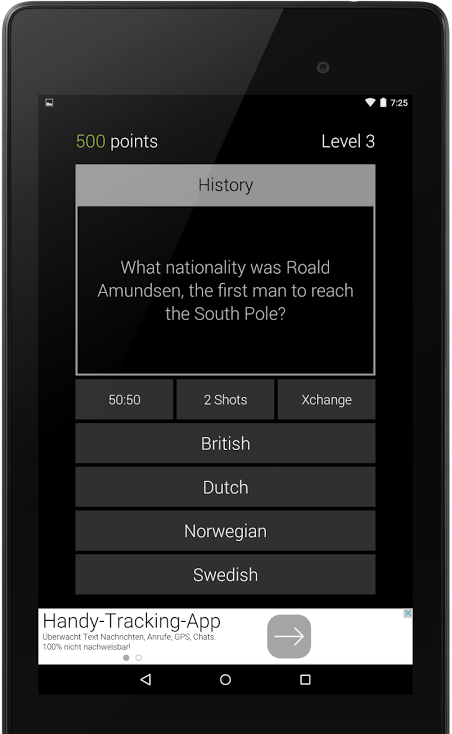
\includegraphics[width=0.7\textwidth]{quizoid.png}
        \caption{Quizoid is a simple multiple-choice game \citep{quizoid}, tested by coaches in iteration 1}.
        \label{fig:quizoid}
    \end{figure}

    \begin{figure}[h]
        \centering
        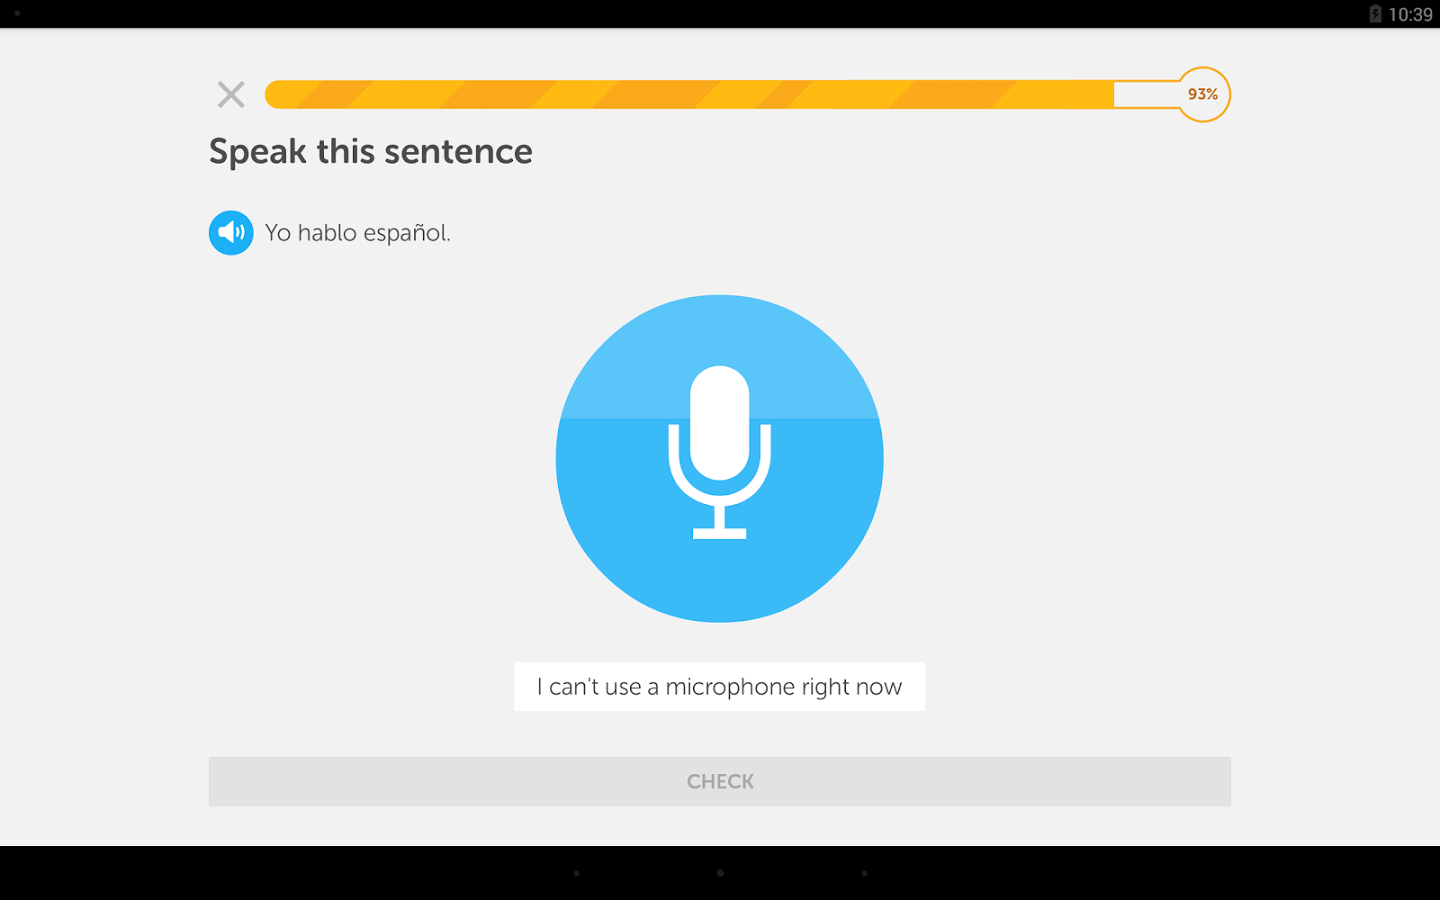
\includegraphics[width=0.7\textwidth]{duolingo.png}
        \caption{Duolingo is a praised app for language learning \citep{duolingo}, tested by coaches in iteration 1}.
        \label{fig:duolingo}
    \end{figure}

    \begin{figure}[h]
        \centering
        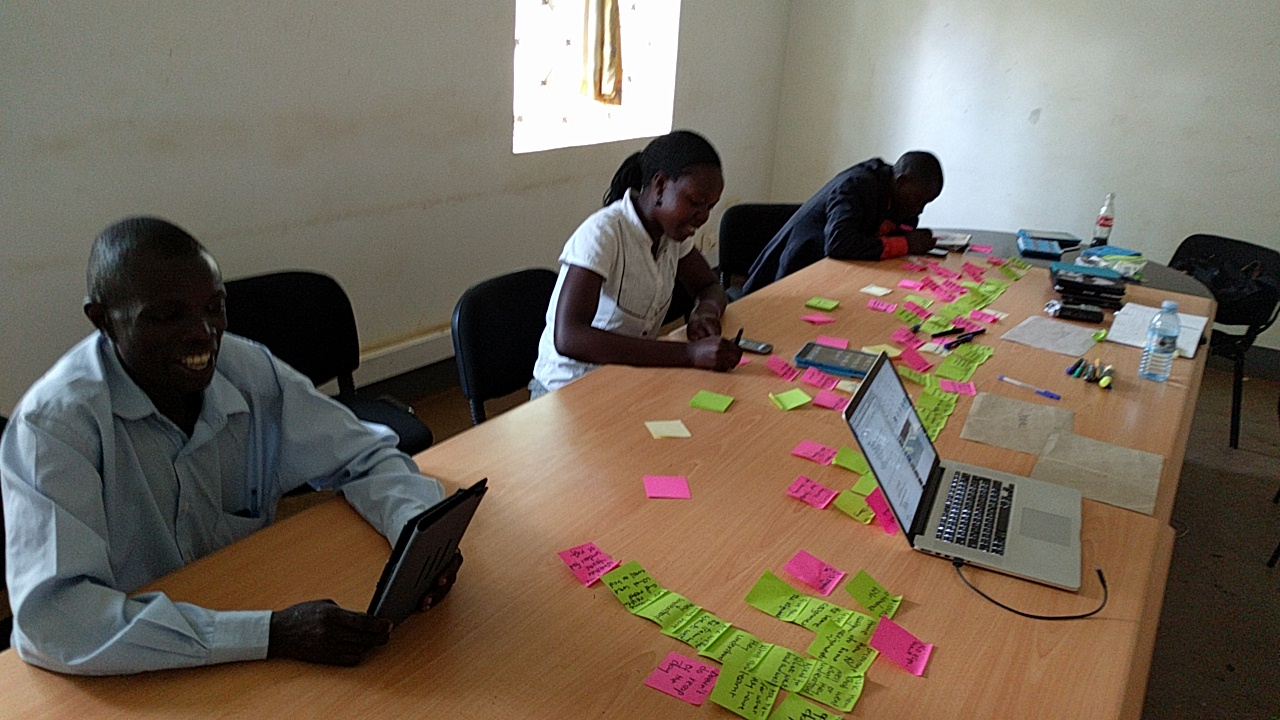
\includegraphics[width=0.7\textwidth]{iteration1/smartphoneTest.jpg}
        \caption{Picture from the smartphone test, observing how the coaches act using Duolingo and Quizoid}.
        \label{fig:smartphoneTest}
    \end{figure}

    Two of the three test users used a smartphone for the first time. The attitude towards using a smartphone was overwhelmingly positive. One of the coaches even mentioned: "Marcus, today one of my dreams have gone true." He even asked if he could borrow one of the devices during the remainder of the stay. Even for coaches that had never touched a smartphone before, some concepts were easily understood (like using the camera and Quizoid).

    Other concepts were harder (accidently getting to the settings menu, unlocking the device, understanding advanced games, or training languages using Duolingo with advanced interactions). Point and click is easily understood, whereas sliding is much more unnatural.

    The result was that the app can place itself somewhere in the middle of the two, regarding difficulty level.
